\documentclass{beamer}

\title{Minimal rational interpolation for \\
       time-harmonic Maxwell's equations}
\date{June 24, 2022}
\author{Fabio Matti}

\usetheme{Minimal}

\begin{document}

\begin{frame}[noframenumbering]

    \titlepage

\end{frame}

\begin{frame}{Outline}

    \begin{itemize}
        \item<1-> Problem formulation
        \item<2-> Finite element approximation
        \item<3-> Minimal rational interpolation
        \item<4-> Example applications
        \item<5-> Conclusion and outlook
    \end{itemize}

\end{frame}

\begin{frame}{Problem formulation}

    Time-harmonic vector potential $\mathbf{u}(\mathbf{x}, t) = \mathbf{u}(\mathbf{x})\exp(i \omega t)$.

    \begin{align*}
        \mathbf{B} &= \nabla \times \mathbf{u} &\text{(Magnetic field)}\\
        \mathbf{E} &= - i \omega \mathbf{u} &\text{(Electric field)}
    \end{align*}

    \begin{block}<2->{Time-harmonic potential equation}
        
        \begin{equation}
            \nabla \times (\mu^{-1} \nabla \times \mathbf{u}) - \epsilon \omega^2 \mathbf{u} = \mathbf{j}
            \label{equ:gauss-bonnet}
        \end{equation}

    \end{block}

\end{frame}

\begin{frame}{Example applications}

    \begin{figure}
        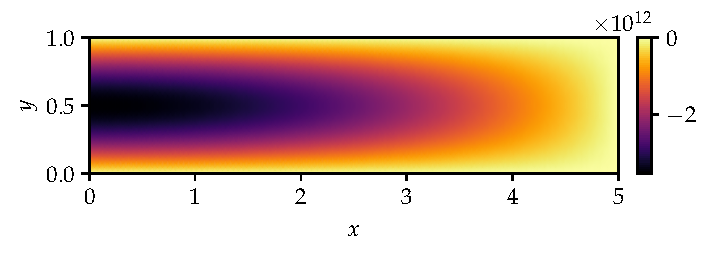
\includegraphics[scale=0.9]{../report/plots/rectangular_cavity_mode1.pdf}
    \end{figure}
    \vspace{-30pt}
    \begin{figure}
        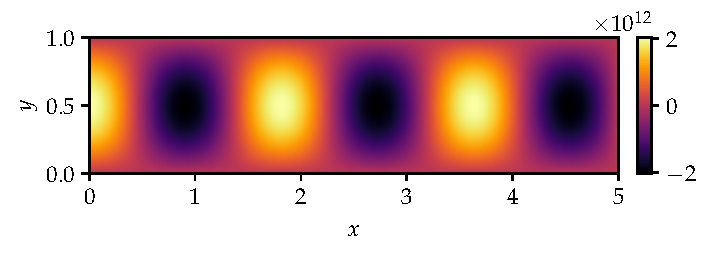
\includegraphics[scale=0.9]{../report/plots/rectangular_cavity_mode5.pdf}
    \end{figure}

\end{frame}

\end{document}